\documentclass[mathserif]{beamer}
%\documentclass[mathserif,handout]{beamer}

%\usepackage{algorithm2e}
\usepackage{mathtools}
\usepackage{booktabs}
\usetheme{metropolis}
%\mode{presentation}

\DeclareMathOperator{\struckDelta}{\Delta \left( \mathbf{y}, \mathbf{y}_i \right)}
\DeclareMathOperator*{\argmax}{arg\,max}
\DeclareMathOperator{\st}{\text{s.t.} \quad}

% front matter
\title{Struck}
\subtitle{Structured Output Tracking with Kernels}
\author{Brendan Robeson}
\date[CS 7680]{CS 7680 - Advanced Computer Vision}
\institute{Utah State University}

\begin{document}
\begin{frame}
    \titlepage
\end{frame}

\begin{frame}
    \frametitle{Outline}
    \tableofcontents
\end{frame}

% each section is in a separate LaTeX file
\section{Tracking by Detection}

\begin{frame}
    \frametitle{How do we track an object from frame to frame?}
    \begin{columns}[T]
        \begin{column}{0.5\textwidth}
            \begin{figure}
                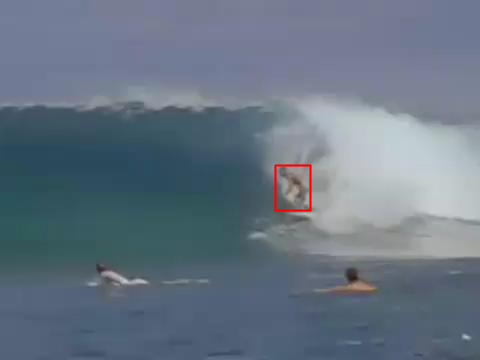
\includegraphics[width=0.9\textwidth]{surfer_marked}
                \caption{Initial frame: The surfer location is known.}
            \end{figure}
        \end{column}
        \begin{column}{0.5\textwidth}
            \begin{figure}
                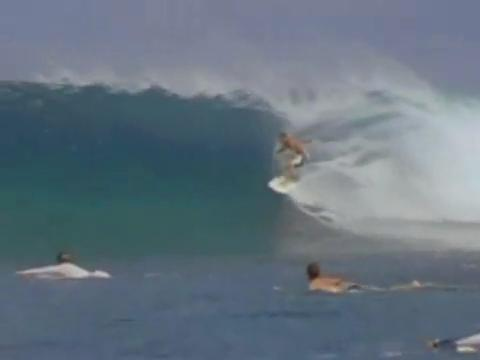
\includegraphics[width=0.9\textwidth]{surfer_unmarked}
                \caption{Subsequent frame: Where is the surfer?}
            \end{figure}
        \end{column}
    \end{columns}
\end{frame}

\begin{frame}
    \frametitle{Tracking can be treated as an object detection problem.}
    \begin{columns}[T]
        \begin{column}{0.5\textwidth}
            \begin{description}
                \item [Tracking by detection] Attempt to detect the object in each frame.
                %\item [Adaptive tracking by detection] Update the classifier online.
            \end{description}
            \begin{itemize}
                \item Transform a tracking problem into an object detection problem.
                \item Can use prior knowledge to assist the detection.
                \item For example, in the previous frame, the object was here. In this frame, it's
                    unlikely to be way over there.
            \end{itemize}
        \end{column}
        \begin{column}{0.5\textwidth}
            \begin{itemize}
                \item The algorithm operates on frame \(f_t\), for \(t \in \{1, 2, ..., T\}\).
                \item Sample \(f_t\) around position \(\vec{p}_{t-1}\).
                \item Extract features \(\vec{x}_i\) for each sample.
                \item Input features to a classifier.
                \item Classifier determines which feature corresponds to the tracked object.
                \item Determine new position \(\vec{p}_t\).
                \item Retrain the classifier with new features. \alert{optional}
            \end{itemize}
        \end{column}
    \end{columns}
\end{frame}

\begin{frame}
    \frametitle{Proposal: Fuzzy Struck}
    \begin{itemize}
        \item Fuzzy SVM incorporates fuzzy logic membership into an SVM. \cite{991432}
        \item Struck uses a structured output SVM. \cite{6126251} \cite{Schwenker2014}
        \item Overall, best performance in a recent survey. \cite{6671560}
        \item Two issues:
            \begin{itemize}
                \item Training samples often contain some object features and some background
                    features.
                \item Target object can change appearance over time, but this is not considered in
                    Struck.
            \end{itemize}
        \item Combine fuzzy SVM with Struck's SVM.
    \end{itemize}
\end{frame}

\documentclass[mathserif,handout]{beamer}
\usepackage{algorithm2e}
%\documentclass{beamer}
\usepackage{booktabs}
\usetheme{metropolis}
%\mode{presentation}

\DeclareMathOperator*{\argmax}{arg\,max}

% front matter
\title{Struck}
\subtitle{Structured Output Tracking with Kernels}
\author{Brendan Robeson}
\date[CS 7680]{CS 7680 - Advanced Computer Vision}
\institute{Utah State University}

\begin{document}
\begin{frame}
    \titlepage
\end{frame}

\begin{frame}
    \frametitle{Outline}
    \tableofcontents
\end{frame}

\section{The Problem}

\begin{frame}
    \frametitle{Tracking can be treated as an object detection problem.}
    \begin{description}
        \item [Tracking by detection] Object detection in each frame.
        \item [Adaptive tracking by detection] Update the classifier online.
    \end{description}

    Separates sample generation from classifier updating.
\end{frame}

%\begin{frame}
%    \frametitle{So, what's wrong with the previous algorithms?}
%    \begin{enumerate}
%        \item<1-> How should samples be generated and labeled?
%
%            \uncover<2->{\alert{Most consider samples far from the target to be negative.}}
%        \item<1-> Classifier wants to determine \emph{what} an object is.
%
%            Tracker wants to determine \emph{where} an object is.
%
%            \uncover<3->{\alert{The two are not trained together. Thus, assuming highest classifier
%            output $\Rightarrow$ location is not always true.}}
%    \end{enumerate}
%    \uncover<4->{Most trackers try to make the classifier more robust with respect to poor samples.}
%\end{frame}

%\begin{frame}
%    \frametitle{Adaptive tracking-by-detection algorithm}
%    \begin{algorithm}[H]
%        \DontPrintSemicolon
%        \KwIn{Video frame: $f_t$}
%            \ForEach{ROI image}
%            {
%                Calculate the GLCM $P_u$\;
%                Calculate energy using Equation (2)\;
%                Calculate contrast using Equation (3)\;
%                Calculate correlation using Equation (4)\;
%                Calculate entropy using Equation (5)\;
%                Calculate homogeneity using Equation (6)\;
%            }
%            \KwOut{A set of feature vectors}
%    \end{algorithm}
%\end{frame}

\begin{frame}
    \frametitle{How does one train adaptive tracking-by-detection?}

    \begin{itemize}
        \item The algorithm operates on frame $f_t$, for $t \in \{1, 2, ..., T\}$.
        \item The tracker estimates a bounding box position, $\mathbf{p}$.
        \item Extract features $\mathbf{x}_t^\mathbf{p}$ from patches within the bounding box.
        \item Train the classifier with $(\mathbf{x}, z)$\uncover<3->{, where $z = \pm1$.}
    \end{itemize}

    \uncover<2>{\alert{What is $z$?}}
\end{frame}

\begin{frame}
    \frametitle{How does one predict using adaptive tracking-by-detection?}

    \begin{itemize}
        \item The goal is to estimate a transformation $\mathbf{y}_t \in
            \mathcal{Y}$, where $\mathbf{p}_t = \mathbf{p}_{t-1} \circ \mathbf{y}_t$.
        \item $\mathcal{Y}$ is the search space in the image.
        \item Typically, $\mathcal{Y} = \left\{ (u,v) | u^2 + v^2 < r^2 \right \}$
            \alert{$\Leftarrow$ What does this mean?}
        \item $\mathbf{y}_t = \argmax\limits_{y \in \mathcal{Y}} h \left(
            \mathbf{x}_t^{\mathbf{p}_{t-1}}, \mathbf{y} \right)$
        \item Uses a classification confidence function $h(\mathbf{x})$
    \end{itemize}
\end{frame}

\begin{frame}
    \frametitle{How does one update the classifier?}

    \begin{itemize}
        \item Update the classifier after calculating $\mathbf{p}_t$.
        \item Generate sample transformations: $\left\{ \mathbf{y}_t^1,
            \mathbf{y}_t^2, ..., \mathbf{y}_t^n \right\}$.
        \item Generate training samples: $\left\{
                \mathbf{x}_t^{\mathbf{p}_t \circ \mathbf{y}_t^1},
                \mathbf{x}_t^{\mathbf{p}_t \circ \mathbf{y}_t^2}, ...,
                \mathbf{x}_t^{\mathbf{p}_t \circ \mathbf{y}_t^n} \right\}$.
        \item Generate labels: $\left\{ z_t^1, z_t^2, ..., z_t^n \right\}$.
        \item Use the samples and labels to update the classifier.
    \end{itemize}
\end{frame}

\begin{frame}
    \frametitle{How to label a transformation.}
    Use a transformation similarity function:

    \begin{equation}
        s_{\mathbf{t}_t}^o \left( \mathbf{y}_t^i, \mathbf{y}_t^j \right) =
            \frac{\left( \mathbf{p}_t \circ \mathbf{y}_t^i \right) \cap \left( \mathbf{p}_t \circ \mathbf{y}_t^j \right)}
                 {\left( \mathbf{p}_t \circ \mathbf{y}_t^i \right) \cup \left( \mathbf{p}_t \circ \mathbf{y}_t^j \right)}
    \end{equation}

    Then, use a labelling function:

    \begin{equation}
        l\left( s_{\mathbf{p}_t}\left(\mathbf{y}^0, \mathbf{y}_t^i \right) \right) =
            \begin{cases}
                +1 & s_{\mathbf{p}_t}\left(\mathbf{y}^0, \mathbf{y}_t^i \right) > \theta_u \\
                -1 & s_{\mathbf{p}_t}\left(\mathbf{y}^0, \mathbf{y}_t^i \right) < \theta_l \\
                 0 & \text{otherwise}
            \end{cases}
    \end{equation}
\end{frame}

\begin{frame}
    \frametitle{So what's wrong with this?}

    \begin{itemize}
        \item $(\mathbf{x}, z)$ does not correlate $\mathbf{y}$ with $z$.
        \item Training samples all have equal weight in the classifier.
            \begin{itemize}
                \item A background sample with significant overlap: $z = -1$.
                \item A background sample with less overlap: $z = -1$.
                \item This leads to tracking error growing over time.
            \end{itemize}
        \item The labeller, and the learner, are distinct.
            \begin{itemize}
                \item Errors by the labeller are noise in the learner.
                \item Current techniques attempt to make the learner more
                    robust, but not address the cause of the noise.
            \end{itemize}
    \end{itemize}
\end{frame}

%\section{Prior Solutions}

\section{Struck}

\begin{frame}
    \frametitle{Here's the gist...}

    \begin{itemize}
        \item Don't learn a binary classifier. Learn a prediction function: $f :
            \mathcal{X} \rightarrow \mathcal{Y}$.
        \item Labelled sample is $(\mathbf{x}, \mathbf{y})$.
        \item $f$ is learned in a structured output SVM.
        \item Use a discriminant function $F: \mathcal{X} \times \mathcal{Y}
            \rightarrow \mathbb{R}$.
        \item Prediction function becomes %\uncover<1>{
            \begin{align}
                \mathbf{y}_t &= \argmax\limits_{y \in \mathcal{Y}} h \left( \mathbf{x}_t^{\mathbf{p}_{t-1}}, \mathbf{y} \right) \tag{prior} \\
                \mathbf{y}_t &= \argmax\limits_{y \in \mathcal{Y}} F \left( \mathbf{x}_t^{\mathbf{p}_{t-1}}, \mathbf{y} \right) \tag{Struck}
            \end{align}
    \end{itemize}
\end{frame}

\begin{frame}
    \frametitle{What is the discriminant function, $F$?}
    \begin{equation}
        F(\mathbf{x}, \mathbf{y}) = \langle \mathbf{w}, \mathbf{\Phi}(\mathbf{x}, \mathbf{y}\rangle
    \end{equation}
    \begin{equation}
        \min_{\mathbf{w}} \frac{1}{2} \|\mathbf{w}\|^2 + C \sum_{i=1}^n \xi_i
    \end{equation}

    Subject to:

    \begin{align}
        \forall i &: \xi \ge 0 \\
        \forall i, \forall \mathbf{y} \ne \mathbf{y}_i &: \langle \mathbf{w}, \delta \mathbf{\Phi}_i (\mathbf{y}) \rangle \ge \Delta (\mathbf{y}_i, \mathbf{y}) - \xi_i
    \end{align}

    \begin{equation}
        \delta \mathbf{\Phi}_i (\mathbf{y}) = \mathbf{\Phi}(\mathbf{x}_i, \mathbf{y}_i) - \mathbf{\Phi}(\mathbf{x}_i, \mathbf{y})
    \end{equation}
\end{frame}

\begin{frame}
    \frametitle{What is the discriminant function, $F$}
    \begin{itemize}
        \item $\Delta$ is a loss function.
            \begin{itemize}
                \item $\Delta (\mathbf{y}, \mathbf{\bar{y}}) = 0 \; \text{iff} \; \mathbf{y} = \mathbf{\bar{y}}$
                \item $\Delta$ should decrease to 0 as $\mathbf{y}$ approaches $\mathbf{\bar{y}}$
            \end{itemize}
        \item This overcomes the equal treatment of samples.
        \item The authors use bounding box overlap:
    \end{itemize}
    \begin{equation}
        \Delta(\mathbf{y}, \mathbf{\bar{y}}) = 1 - s_{\mathbf{p}_t}^o (\mathbf{y}, \mathbf{\bar{y}})
    \end{equation}
\end{frame}

%\begin{frame}
%    \frametitle{How does Struck work?}
%    \begin{itemize}
%        \item Learning and tracking are integrated.
%        \item Uses a structured output SVM.
%        \item Must overcome the \alert{curse of kernelization.}
%            \begin{itemize}
%                \item Number of support vectors increase as a function of training data
%            \end{itemize}
%    \end{itemize}
%\end{frame}

\section{Experiments}

\begin{frame}
    \frametitle{How did they measure performance?}
    \begin{block}{Bounding box overlap}
        $\text{IoU} = \frac{B \cap G}{B \cup G}$
    \end{block}
\end{frame}

\begin{frame}
    \frametitle{Bounding box overlap}
    \begin{tabular}{l c c c c }
        \toprule
        Video & Struck\textsubscript{$\infty$} & Struck\textsubscript{100} & Struck\textsubscript{50} & Struct\textsubscript{20} \\
        \midrule
        Coke      & \textbf{0.57} & \textbf{0.57} &         0.56  & \underline{0.52} \\
        David     &         0.80  &         0.80  & \textbf{0.81} &            0.35  \\
        Face 1    &         0.86  &         0.86  &         0.86  &            0.81  \\
        Face 2    & \textbf{0.86} & \textbf{0.86} & \textbf{0.86} & \underline{0.83} \\
        Girl      & \textbf{0.80} & \textbf{0.80} & \textbf{0.80} & \underline{0.79} \\
        Sylvester & \textbf{0.68} & \textbf{0.68} &         0.67  &            0.58  \\
        Tiger 1   & \textbf{0.70} & \textbf{0.70} &         0.69  & \underline{0.68} \\
        Tiger 2   &         0.56  & \textbf{0.57} &         0.55  &            0.39  \\
        \bottomrule
    \end{tabular}
\end{frame}

\begin{frame}
    \frametitle{Bounding box overlap}
    \begin{tabular}{l c c c c c c }
        \toprule
        Video & Struck & MIForest & OMCLP & MIL & Frag & OAB \\
        \midrule
        Coke      & \textbf{0.57} & 0.35 & 0.24 & 0.33 &         0.08  & 0.17 \\
        David     & \textbf{0.81} & 0.72 & 0.61 & 0.57 &         0.43  & 0.26 \\
        Face 1    &         0.86  & 0.77 & 0.80 & 0.60 & \textbf{0.88} & 0.48 \\
        Face 2    & \textbf{0.86} & 0.77 & 0.78 & 0.68 &         0.44  & 0.68 \\
        Girl      & \textbf{0.80} & 0.71 & 0.64 & 0.53 &         0.60  & 0.40 \\
        Sylvester & \textbf{0.68} & 0.59 & 0.67 & 0.60 &         0.62  & 0.52 \\
        Tiger 1   & \textbf{0.70} & 0.55 & 0.53 & 0.52 &         0.19  & 0.23 \\
        Tiger 2   & \textbf{0.57} & 0.53 & 0.44 & 0.53 &         0.15  & 0.28 \\
        \bottomrule
    \end{tabular}

    The Struck column shows the best values from the previous table.
\end{frame}

\begin{frame}
    \frametitle{Processing time}
    \begin{tabular}{l c c c c }
        \toprule
        Video & Struck\textsubscript{$\infty$} & Struck\textsubscript{100} & Struck\textsubscript{50} & Struct\textsubscript{20} \\
        \midrule
        Average FPS & 12.1    & 13.2    & 16.2    & 21.4 \\
        %Average SPF &  0.0826 &  0.0758 &  0.0617 &  0.0467 \\
        \bottomrule
    \end{tabular}

    Not keeping up with typical U.S. frame rate!
\end{frame}

%\begin{frame}
%    \frametitle{Combining kernels}
%    \begin{tabular}{l c c c c c c }
%        \toprule
%        Video & Struck & MIForest & OMCLP & MIL & Frag & OAB \\
%        \midrule
%        Coke      & \textbf{0.57} & 0.35 & 0.24 & 0.33 &         0.08  & 0.17 \\
%        David     & \textbf{0.81} & 0.72 & 0.61 & 0.57 &         0.43  & 0.26 \\
%        Face 1    &         0.86  & 0.77 & 0.80 & 0.60 & \textbf{0.88} & 0.48 \\
%        Face 2    & \textbf{0.86} & 0.77 & 0.78 & 0.68 &         0.44  & 0.68 \\
%        Girl      & \textbf{0.80} & 0.71 & 0.64 & 0.53 &         0.60  & 0.40 \\
%        Sylvester & \textbf{0.68} & 0.59 & 0.67 & 0.60 &         0.62  & 0.52 \\
%        Tiger 1   & \textbf{0.70} & 0.55 & 0.53 & 0.52 &         0.19  & 0.23 \\
%        Tiger 2   & \textbf{0.57} & 0.53 & 0.44 & 0.53 &         0.15  & 0.28 \\
%        \bottomrule
%    \end{tabular}
%\end{frame}

\section{Conclusion}

\begin{frame}
    \frametitle{References}
    \nocite{*}
    \bibliographystyle{IEEEtran}
    \bibliography{references}

    Source code: \url{https://github.com/samhare/struck}
\end{frame}

\end{document}


\section{Experiments}

\begin{frame}
    \frametitle{Data sets}
    \url{http://vision.ucsd.edu/~bbabenko/project_miltrack.html}
    \begin{itemize}
        \item Eight sequences used in \cite{6126251}.
        \item Ensure I didn't make it worse.
    \end{itemize}
    \url{http://alov300.org/}
    \begin{itemize}
        \item 314 sequences used in \cite{6671560}.
        \item Categorized to test various object tracking challenges.
    \end{itemize}
\end{frame}

\begin{frame}
    \frametitle{Experimental Setup - Struck}
    \begin{itemize}
        \item Set up as described in their paper:
            \begin{itemize}
                \item Haar features
                \item Gaussian kernel \(\sigma\) = 0.2
                \item \(C\) = 100
                \item Search radius \(r\) = 30 pixels
                \item SVM budget = 100
            \end{itemize}
        \item Unknown parameters - Unmodified from the configuration in the repository:
            \begin{itemize}
                \item Frame size - set to 320 x 240
                \item Random seed - set to \(\{0, 1, 2, 3, 4 \}\)
            \end{itemize}
    \end{itemize}
\end{frame}

\begin{frame}
    \frametitle{Experimenting vs Struck}
    \begin{algorithm}[H]
        \DontPrintSemicolon
        \KwIn{Sequences}
        \Begin(Run experiment)
        {
            \ForEach{Sequence}
            {
                \ForEach{Random seed}
                {
                    Run Struck\;
                    Compare with ground truth\;
                    Record mean IoU\;
                }
                Report median of mean IoU's\;
            }
        }
        \KwOut{IoU results}
    \end{algorithm}
\end{frame}

\begin{frame}
    \frametitle{Bounding box overlap results}
    \begin{center}
        \begin{tabular}{l c c c }
            \toprule
            Video & Struck\textsubscript{\cite{6126251}} & Struck\textsubscript{Mine} & Fuzzy Struck \\
            \midrule
            Coke      &         0.57  & \textbf{0.88} & TBD \\
            David     &         0.80  & \textbf{0.86} & TBD \\
            Face 1    & \textbf{0.86} & \textbf{0.86} & TBD \\
            Face 2    & \textbf{0.86} &         0.80  & TBD \\
            Girl      & \textbf{0.80} &         0.68  & TBD \\
            Sylvester &         0.68  & \textbf{0.86} & TBD \\
            Tiger 1   & \textbf{0.70} &         0.67  & TBD \\
            Tiger 2   &         0.57  & \textbf{0.67} & TBD \\
            \bottomrule
        \end{tabular}
    \end{center}
\end{frame}


\section{Conclusion}

\begin{frame}
    \frametitle{What does Struck do?}
    Struck provides an adaptive tracking-by-detection framework.

    It directly ties image features to a transformation.

    It eliminates binary labelling with equal weight.

    It uses a structured output SVM, with a boundary on the number of support vectors.
\end{frame}

\begin{frame}
    \frametitle{Where does Struck fall short?}
    Currently, Struck focuses solely on translation.

    Though rotation does not appear to confuse Struck, it's not detected and shown.

    Smeulders et. al. concluded Struck's primary problem was dealing with scale (camera zoom).
\end{frame}

\begin{frame}
    \frametitle{References}
    \nocite{*}
    \bibliographystyle{IEEEtran}
    \bibliography{references}

    Source code: \url{https://github.com/samhare/struck}
\end{frame}


\end{document}

